\chapter{相对论激光与临界密度等离子体作用中的成丝不稳定性}
\label{chap:instability}



\section{简介}
等离子体本身是一个复杂的系统,稳定性的研究是其很重要的方向。简单的模型来描述稳定性,正如\ref{fig:stable}所示。假设,存在微小的扰动使得系统偏离平衡状态,稳态系统中,系统通过负反馈及时地平衡扰动,使得系统回复到平衡状态;而对于非稳定系统,  而这种偏离对于非平衡产生正反馈从而加剧了不平衡的程度,使之增长,并最终形成 一种明显效应离开平衡态。
\begin{figure}[!htbp]
  \centering
  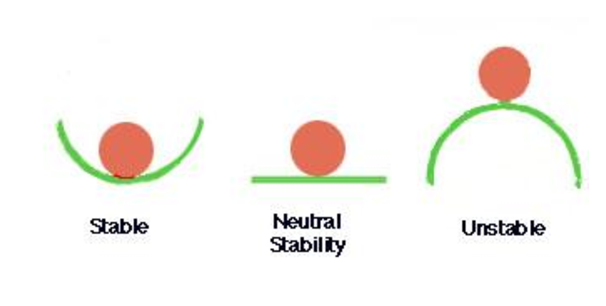
\includegraphics[width=\MyFactor\textwidth]{Img/stable.eps}
  \caption{平衡状态}
  \label{fig:stable}
\end{figure}



 不稳定的形成和增长对于研究激光在等离子体中的吸收,能量沉积,以及热电子的传输等,都有很重要的意义,在快点火聚变\cite{tabak1994ignition},天体物理中有广泛的应用,同时在离子加速中也有重要的影响。等离子体中存在不计其数不稳定性,我们侧重于激光与质密厚靶($\mu m$以上)作用过程中不稳定性的研究。由于激光无法穿透等离子体并在其中传播,因此激光传输过程中的不稳定性就不需要考虑,而激光在等离子体前表面产生的电流向后传播的过程中,存在非常多的不稳定性。
其中常见的流布稳定性包括的有: 韦伯不稳定性\cite{weibel1959spontaneously},双流不稳定性等。韦伯不稳定性,发生在均匀或者近均匀等离子体中。由于电子在动量空间中各向异性分布,通常可以简化理解为不同方向上的两种温度。在微小的磁场扰动下,不同温度的电子产生不同的偏移而产生电流,而这种电流会产生磁场进一步增强原磁场,促进这种扰动并导致不稳定性的增长,最终出现明显的不稳定性的现象。双流不稳定性,是等离子体中常见的现象。当高能粒子束流在等离子体中传播时,电子和离子束流具有不同的速度,而这种不同速度分布会激发等离子体波以及不稳定性。如图\ref{fig:twoStream},当高能电子束流入射到等离子体中,其速度分布出现一个局部的凸起。如果一种等离子体波的相速度处于如图所示的位置,则大于相速度的‘快电子’数目要多于‘慢电子’,粒子的能量将转化至此等离子体波中。

\begin{figure}[!htbp]
  \centering
  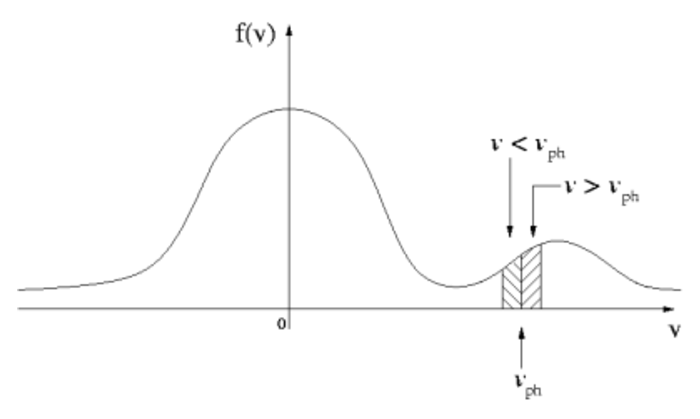
\includegraphics[width=\MyFactor\textwidth]{Img/twoStream.eps}
  \caption{双流不稳定性}
  \label{fig:twoStream}
\end{figure}


当激光与等离子体前表面产生的高能电子正向电流在等离子体中传播时,由于电中性的要求,背景电子存在回流。这种回流与正向电流方向相反,并由此激发与电流的方向垂直的成丝分布,而这一现象和以上三种不稳定性相关。如图\ref{fig:Bret2005}\cite{bret2005characterization},其中成丝不稳定性与韦伯不稳定性属于不稳定性增长方向与扰动方向垂直的横向模式,双流不稳定性属于纵向模式。在非相对论领域,双流不稳定性处于主要的地位;而对于相对论电流,成丝不稳定性占据主导地位。然而在成丝的过程中,各种模式共同存在,并通过偶和的方式决定了不稳定性的增长率等。

\begin{figure}[!htbp]
  \centering
  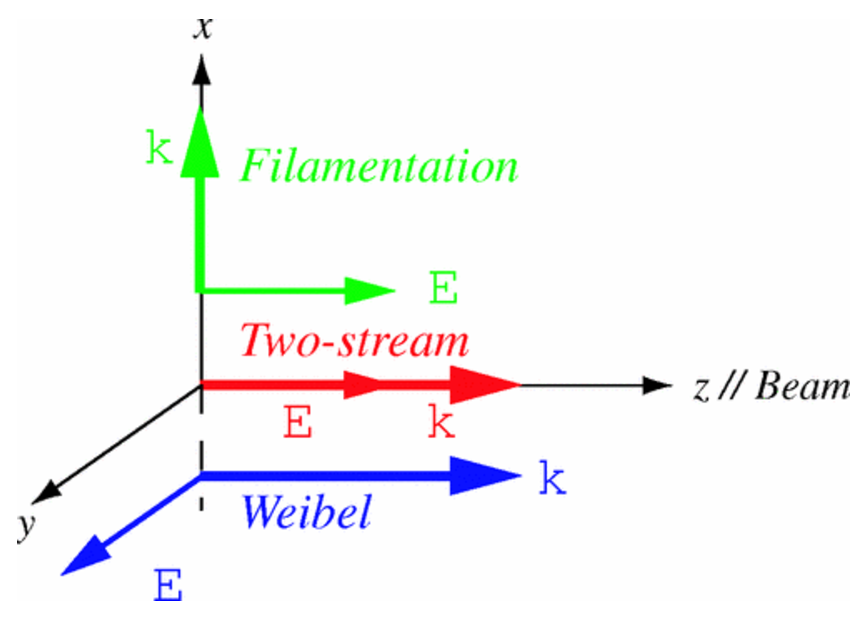
\includegraphics[width=\MyFactor\textwidth]{Img/Bret2005.eps}
  \caption{成丝过程中的不稳定模式}
  \label{fig:Bret2005}
\end{figure}

基于无限空间中高能电子束流在等离子体中的传播模型,A. Bret\cite{bret2005characterization,bret2004collective}研究了三种模式共同存在下,成丝不稳定性的增长率以及成丝具体分布的研究,得出如下结论。
\begin{equation}
\label{eqn:maxGrowth}
{\sigma}_M= \frac{\sqrt{3}}{2^{4/3}}(\frac{\alpha}{{\gamma}_b})^{1/3} {\omega}_p
\end{equation} 
其中${\sigma}_M$是最大增长率,$\alpha=n_b/n_p$,$n_b$是回流的密度,$n_p$是正向电流的密度,${\gamma}_b=1/sqrt{1-{\beta}^2}$,$\beta=V_b/c$,${\omega}_p=(4 \pi n_p e^2/m_e)^{1/2} $是等离子体频率。

\begin{equation}
\label{eqn:filamentSpace}
L_f \approx \pi {\lambda}_s \sqrt{V_{tp}/V_b}
\end{equation} 

其中$L_f$是成丝间隔,$V_{tp}$是前向电流的速度, $V_b$是回流的速度。


然而在激光与有限厚度等离子体作用的过程中,高能电子束流在等离子体中的传播情况出现了变化。由于靶厚有限,电子回流会产生影响,不稳定性的增长率以及成丝分布情况发生的变化。由此使得电子的分布受到影响,电子在靶后表面相应的形成的鞘层场也有一定的变化,最终影响了出射离子的分布。




\section{强电流在等离子体中的成丝现象}

1 相对论电流的产生分析
相对论激光与近临界密度的等离子相互作用的时,由于激光可以穿透靶,使得作用时间与作用距离增加,激光与等离子体的能量转换效率得到显著的提高。其中比较直接的效果,是电流的增强,由于单位时间内产生的热电子的数目要高于激光与金属靶作用过程,其电流往往高于阿尔芬电流极限,对应于$1MeV$, 阿尔芬极限为$17kA$。


2 阿尔芬电流极限以及等离子体中电流回馈作用
阿尔芬极限是真空中电流传播的极限电流值。当电流在真空中传播时,电流中的电子会受到电流自生磁场以及电子间库伦排斥共同作用,这种影响与电流强度存在一定的关系。当电流强度高于一定值的时候,自生磁场的作用处于主导地位,电子受到磁场作用产生强烈的回转作用,阻碍电流的进一步传播。但是在等离子体中,情况不同于真空中的情况。因为等离子中的准中性要求,因此在存在电流的部分,有相应的回馈电流,保证局部的电荷守恒关系。而且正是由于这种电流回馈的机制使得相对论强度的电流可以传播。例如,当$a=50$强度激光在50$N_c$等离子体中传播时候,产生的电流的强度为$50kA$,远超出阿尔芬电流极限,然而由于局部的回馈电流的存在,这种电流的传播成为可能。回馈电流的分布是一种等离子体被动相应电荷移动的方式,因此回馈电流的分布很大程度上是有传播电流的分布决定的。相对于传播电流,回馈电流存在以下的特点:
1 组成电子为背景电子
2 密度相对较高
3 电子平均速度相对较低



3 回馈电流对于不稳定性的影响的分析

这是由于回馈电流的存在,相对论电子电流在等离子体中传播的过程中,存在着不稳定的模式。强电流在等离子体中传播是,通常存在三种不稳定性,韦伯不稳定性,双流不稳定性,以及纵向成丝不稳定性。三种不稳定性,韦伯不稳定性的出现是由于电子的温度分布存在某个方向上的优势,而这种温度优势可以通过微小的扰动得到增长放大,从而建立起不稳定的模式。双流不稳定性是由于电子与离子双流之间由于想速度与波速之间的不同存在着能量的吸收与释放的过程,伴随于此的不稳定性现象。而成丝不稳定性,产生的原因正是由于传播电流以及回馈电流的相对传播,微扰即可使得电流的分布产生中的变化。从物理机制上看,韦伯不稳定性与成丝不稳定性是一种机制,但是由于韦伯不稳定性的存在于非相对论的情况,成丝不稳定性在相对论的情况下较多。因为电子回流效应对于不稳定性的影响,在相对论电流的情况下比较的明显。
理论上可以通过色散关系的分析此过程。我们通过麦克斯韦方程,连续性方程来推导色散关系,并且假设不稳定模式形式为$exp(i (\vec{k} \cdot \vec{r} -\omega t))$,其中k为波数矢量,$\omega$为不稳定性的频率。为了简化推导,我们采用韦伯不稳定性研究中常用的坐标系设置,其中传播电流的方向为$\vec{z}$,不稳定性的增长方向为$\vec{x}$,磁场的方向为$\vec{y}$。
首先使用电磁场的旋度方程得到电场的传播方程:


\begin{equation}
\vec{\nabla} \times ( \vec{\nabla} \times \vec{E})= - \vec{\nabla} \times \frac{ \partial{\vec{B}}}{\partial{t}}
\end{equation}


\begin{equation}
\vec{\nabla} \times \vec{B}= \frac{ \partial{\vec{E}}}{\partial{t}} + \vec{J}
\end{equation}


\begin{equation}
\frac{\partial^2}{\partial{t^2}} \vec{E} - \nabla^2{\vec{E}} = - \frac{\partial}{\partial{t}} {\vec{J}}- \vec{\nabla} (\vec{\nabla} \cdot \vec{E})
\end{equation}


电流$ J =e n v$,同时我们假设密度与平均速度具有形式,$n= n_0+n_1$,$v=v_0+v_1$,因此电流的扰动如下:
\begin{equation}
J_1= e(n_1 v_0+ n_0 v_1)
\end{equation}
其中,$v_0$,$n_0$是本征速度与密度,$n_1$和$v_1$是微扰量级。通过连续性方程以及运动方程,我们可以得到$n_1$和$v_1$。

\begin{equation}
m (\frac{\partial{v}}{\partial{t}} + (\vec{v} \cdot \vec{\nabla}) \vec{v}) + e(\vec{E}+ \vec{v} \times \vec{B}) = 0
\end{equation}

\begin{equation}
\vec{\nabla} \times \vec{E}= -\frac{ \partial{\vec{B}}}{\partial{t}}
\end{equation}
首先通过运动方程,使用电场旋度方程消去磁场量得到$v_1$与$E$之间的关系,而后通过连续性方程得到密度扰动$n_1$于电场$\vec{E}$之间的关系。
\begin{equation}
\begin{cases}
\vec{v_{1x}}=\frac{eE_z}{i m {\omega}^2} k v_0 \\
\vec{v_{1y}}= 0 \\
\vec{v_{1z}}=\frac{eE_z}{i m {\omega}}  \\
n_{1}=n_0 \frac{\vec{k} \cdot \vec{v_1}}{\omega}=n_0 \frac{\vec{k}}{\omega} v_{1x} \\
\end{cases}
\end{equation}
其中$\vec{v_{1x}}$,$\vec{v_{1y}}$,$\vec{v_{1z}}$分别为电子平均速度的三个分量。相应的传播电流微扰$\vec{J_{1b}}$,$\vec{J_{1r}}$,以及总的电流微扰$\vec{J_1}$为
\begin{equation}
\begin{cases}
\vec{J_{1b}}= -n_0 \frac{e^2 E_z}{i m {\omega}^2} k v_0 \vec{x} -\frac{n_0 e^2}{i m \omega} E_z (1+\frac{k^2 {v_0}^2}{{\omega}^2}) \vec{z} \\
\vec{J_{1r}}= +n_0 \frac{e^2 E_z}{i m {\omega}^2} k v_0 \vec{x} -\frac{n_0 e^2}{i m \omega} E_z (1+\frac{k^2 {v_0}^2}{{\omega}^2}) \vec{z} \\
\vec{J_1}=-2 \frac{n_0 e^2}{i m {\omega}} (1+\frac{k^2 {v_0}^2}{{\omega}^2}) E_z \vec{z}
\end{cases}
\end{equation}
其中回馈电流的速度微扰与传播电流速度微扰同正负,而密度微扰异号,因此速度微扰决定部分相互增强,密度微扰决定部分相互抵消。最终的电流微扰主要存在于$\vec{x}$方向上。带入以上的变量,我们得到色散关系如下:
\begin{equation}
(k^2 -\frac{{\omega}^2}{c^2}) =  -\frac{{{\omega}^2}_p}{c^2} (1+ \frac{k^2 {v^2_0}}{{{\omega}^2}})
\end{equation}

其中${{\omega}}_p = \sqrt{\frac{2 n_0 e^2}{m  \omega}}$等离子体为趋肤深度。
求解以上的色散方程,得到的关系如下:
\begin{equation}
\omega= i {\omega}_p \frac{v_0}{c} \frac{1}{1+ {{\omega}_p}^2/{k^2c^2}}
\end{equation}
由于频率为虚值,在指数分布中存在$exp{i \omega t}$的增长项。
于是增长率$\gamma={\omega}_p \frac{v_0}{c} \frac{1}{1+ {{\omega}_p}^2/{k^2c^2}}$。 典型波数为 $kc \approx {\omega}_p$,同时如果电流扰动得到一定的增强$J_1=J \times \alpha$,$\alpha > 1$,则色散关系为:
\begin{equation}
\omega= i {\omega}_p \frac{v_0}{c} \frac{\alpha}{\alpha+ {{\omega}_p}^2/{k^2c^2}}
\end{equation}
相应的增长率$\gamma =  \frac{v_0}{c} \frac{\alpha}{\alpha+ {{\omega}_p}^2/{k^2c^2}} {\omega}_p $以及波数为$kc \approx  {\omega}_p / \sqrt{\alpha}$。

对于相向传播电流之间的不稳定性, A. Bret\cite{bret2005characterization,bret2009weibel}得出线性条件下的理论,主要结论是增长率$\gamma$以及不稳定的波长$L_f$:


\begin{equation}
\label{eqn:dispersion}
\begin{cases}
{\gamma} \approx \beta \sqrt{\frac{{\alpha}}{{\gamma}_b}} {\omega}_p   \\
L_f \approx \pi {\lambda}_s \sqrt{V_{tp}/V_b}
\end{cases}
\end{equation}


其中$\beta= V_b/c$,${\gamma}_b = 1/ \sqrt{1-{\beta}^2}$,$\omega_p$是等离子体频率。${\lambda}_s$是等离子体的趋肤深度, $V_{tp}$是回馈电流速度,且$V_b$是传播电流速度。其结果与本文中的结论相一致。



前面提到相对论激光穿透靶的作用过程中,产生的强电流在等离子体中传播,传播电流与相应的回馈电流组成的系统正好是相向传播的电流系统。然而不同之处在于,这其中的反向电流是由等离子体被动响应产生的。而且对于有限厚度的靶子,需要考虑靶与真空分界面的情况,因为超过阿尔芬极限的电流是无法在真空中传播的。当传播电流达到靶后的时候,由于强自生磁场的作用,电子在磁场作用下被反向注入到了等离子体中。而这一部分电流将作为回馈电流的一部分,对于成丝不稳定性产生一定的影响。这一点在\cite{eqn:dispersion}中得以体现,当回馈电流增强时,$\alpha$增大并且增长率$\gamma$增加。于此同时,不稳定性的波长也随之增加。物理现象上的具体变现为,当回馈电流增强的时候,电流丝状分布的间距增加,而且丝的强度增加。



\subsection{PIC模拟以及分析}


仿真的参数基于Helmholz Zentrum Dresden-Rossendorf,Institution of Radiation的Draco激光器参数以及法国工程师制造的40$N_c$最大厚度25micron的氢靶而设计,目的在于研究在激光等离子体相互作用过程中,不稳定性对于出射离子的分布的调制作用。其参数基本如下:激光强度$3.45 \times 10^{21} W/cm^2$(对应于归一化激光电场矢量$a=50$),激光的焦斑大小为5微米,横向和纵向分布都是高斯分布,光脉冲的持续时间为330fs。相应的靶的参数如下:密度$40N_c$,厚度为$25$微米的氢均匀靶。模拟中的PIC参数设定:$4800 \times 2400$ 格点用于解析 $60 \times 30 {\mu m}^2$,每个计算格点中有80个粒子,以保证计算的精度。模拟中的时间单位为$T=3.3fs$,距离单位$\mu m$。相对论强度激光在$25T$的时候达到靶前表面,激光峰值光强在$75T$达到靶前表面。如果假设峰值光强在前表面产生的电流具有光速,强电流在$t=100T$的位置到达靶后表面的位置。由于$a/{n \gamma} > 1$,因此激光可以穿透到靶子的内部,产生热电子以及强电流。其过程可以由hole boring机制描述,本文对其过程不做深入的分析。理论上传播电流具有最高的强度,因此通过自生磁场的偏转作用后,回馈电流的增强效应是最强的。相对于无限厚度的等离子体,靶后表面处的回馈电流增强对于不稳定性有着很重要的影响。


首先,我们分析了靶后附近处的电流分布的情况。由于靶内部的电流分布比较的复杂,传播电流以及回馈电流同时存在,我们选取从靶后表面到之后的数微米之间的距离, 统计其中的电流的横向的电流分布的情况,得到的靶后表面的分布情况如下图所示。电流存在明显地先前与向后方向的间隔分布,由于在系统中不存在从反方向产生和传播的电子源,因此可以断定,向后方向的电子的产生是由于磁场的偏转作用的影响,其中的磁场正是由于强电流到真空之后产生的自生磁场。由于磁场的本身对于电流的影响体现在使得电流的轨迹发生偏转,而无法实现电流的成丝作用,因此成丝的过程是发生在靶子内部的过程。而这种成丝的过程的产生区域可以是在靶子的前表面,后表面以及传播的过程中,为了更好的分析其传播过程,我们采用了两种分析的方法。

对于靶子内部电子的信息进行了相应的统计,将正向的电子以及反方向的电子的运动分开进行统计, 得到的结果中,并且区分电子锁处于的位置。其最终是在后表面附近的位置可以得到明显的电子的成丝的现象,然而在其他位置的情况相对的不明显。另一方面,成丝的电子的密度以及能量相对于背景电子较高,因此可以统计靶内部的能量密度分布以及相应的密度分布的方法对于相应的情况进行好的分析,最终的结论中的很有意义的部分如下:
1 电子的丝状的能量分布发生在接近后表面的位置,而并非是在激光与靶作用的具体位置
密度分布的信息中,由于背景电子的密度比较的高,密度分布的信息中无法得到不稳定性成丝结果的位置分布。


同时丝状不稳定结构的间距比较均匀,可以确定是一种模式起到主导的作用,因此考虑使用信号处理的方法去除噪声信号的影响,得到信号的分布。通过这种方法, 得到的信号的频率为等离子体频率的六分之一。而这与传统的韦伯不稳定性关于不稳定性模式的预测有一定的不同。


之前的关于不稳定性的频率的分析表明,在电流的扰动得到明显的增强的情况下,不稳定模式的波长得到相应的增加,因此这种不同于韦伯不稳定性的模式,很有可能是由于后表面的电流的增强效应产生的结果。为了进一步核实这种结论,统计了正向以及反向电流的分布,希望得到电流的扰动的变化的信息。




最终结论与相应的分析吻合。我们总结如下:
在强相对论激光与临界密度等离子体作用的过程中,激光能量有效的传输至电子,在靶的前表面产生强电流。电流在等离子体中传播,而传播过程中没有激光的参与,可以作为电子束流与等离子体的相互作用。由于等离子体的准电中性你的要求,因此在等离子体中,存在一定的反向回馈电流满足这一条件。正是由于回馈电流的存在,超过阿尔芬极限的电流也可以在等离子体中传播。但是当电流到达靶子的后表面,传输在真空等离子体分界面的时候,由于电流的强度超过阿尔芬极限,在强烈的自生磁场的作用下,一部分低能量的电子改变了方向,重新注入到了靶子中,成为了反向回馈电流的一部分。回馈电流的存在极大的增强了后表面位置处的电流的扰动,使得增长速率相对较慢的不稳定性得到了很大的加强,迅速的增长起来,形成规律的周期性不稳定结果,并且影响了正向传播的电流,对于电流的分布产生了强烈的调制作用。在这种调制作用下,电子的分布以及加速场的分布也收到了很大的影响。而其直接的效果是对于加速离子的分布的影响,使得出射离子束流也存在周期性的结构的存在。这种不稳定性对于加速是有害的,








